\documentclass[a4paper,12pt]{report}

\usepackage[english]{babel}
\usepackage[utf8]{inputenc}
\usepackage[T1]{fontenc}
\usepackage{amsmath}
\usepackage{graphicx}
\usepackage{titlesec}






\titleformat{\chapter}[hang]
  {\normalfont\huge\bfseries}
  {\thechapter\quad} % This is the number (e.g. "1")
  {0pt}
  {} % No label text like "Chapter"







\title{Bachelor's Thesis\\ \
\\
Comparative Study about predictive performance of Machine Learning algorithms in forecasting prices of stocks with different volatility}
\author{Jeremias Lukas Aechtner}
\date{June 29, 2025}

\setcounter{secnumdepth}{6}
\setcounter{tocdepth}{6}






\begin{document}



\maketitle


\section*{Acknowledgment}
First I would like to thank Professor Gregory Provan and Professor Dr. Andreas Maletti who agreed to supervise me on this topic that I wanted to work on so badly. I always received their guidance and honest opinions as an invaluable support for both the development of the content of the thesis and the general process of writing this thesis. I would like to express my sincere gratitude towards my friends and family that supported me in many ways throughout the entire process.
\newpage

\tableofcontents
\newpage






\chapter{Introduction}
ML has become a very important technology in time series forecasting over various fields where researchers apply it to real world challenges. These fields include Healthcare [1], Energy [2], Agriculture [3], Climate and Weather [4] and financial data. Especially in financial data people have a huge interest in making accurate forecasts about developments of for example companies and stock prices given the huge potential for profit in trading. 
In this paper we want to evaluate different Machine Learning models against each other based on their performance of forecasting different stock prices and indices. We therefore observe the current literature in this field:



\chapter{Literature Review}
The paper [5] from Kumbure et al. (2022) showed in a comprehensive review the technological development in the field of stock forecasting. The review includes 138 articles that have been published between 2000 and 2019. It looks on machine learning techniques that have been applied, features that were considered for training and metrices with which results have been measured. Like that they propose a differentiation of features into 4 categories which are “Technical Indicators”, “Macro-Economy”, “Fundamental Indicators” and “others”. They explain the importance and use frequency of these features. In section 5.4.8 that paper [5] illustrates what families of machine learning models have been applied to the task of forecasting stock prices. It shows that at least since the year 2000 Artificial Neural Networks (ANNs) in various forms were experimented with excluding Deep Learning models that are listed separately. That differentiation shows that deep learning models have especially been investigated heavily in the more recent years with the first reviewed paper applying them in 2017. 
One representative of Deep Learning is mentioned very regularly in research – Long Short-Term Memory (LSTM). The paper [6] by Matharasi et al. (2025) evaluates two models against each other which are LSTM and XGBoost. Both delivered promising accuracy in forecasting AMD inc. stock data. While the LSTM model delivered slightly better accuracy in forecasts, the XGBoost model could excel in computational efficiency. Both models have been shown to have outstanding predictive performance when forecasting certain stock or index data. Teixeira, D. M., and Barbosa, R. S. (2025) have conducted another experiment [13] that shows their effectiveness in capturing the complexity of stock prices. They evaluate the models LSTM and XGBoost as well as other architectures such as GRU, CNN, RNN, but also different hybrid combinations of these like LSTM + CNN, RNN + GRU, GRU + CNN, LSTM + GRU, and RNN + LSTM. The study trains all of these models on historical stock data from Apple inc. and comes to the result that the standalone models of GRU, LSTM and XGBoost perform the best for the Apple inc. stock data. This is a little counterintuitive since one might think that hybrid models usually outperform their standalone component models since they might merge strengths of both models but as evidenced that is not generally the case. Under section 5 they discuss that the performance depends furthermore on the timeframe of the training data. They state that the gap of the performance between the models is smaller for a shorter time frame of training data. They state that the reason for that is the lower complexity of that time frame with fewer large amplitude oscillations. When choosing a longer time frame for training with a more complex data course, the three earlier mentioned models GRU, LSTM and XGBoost outperform the other models. Another paper [7] by Li, Siyuan. (2024) investigates the performance of a Kalman Filter and different types of LSTM models such as a single layer LSTM, a stacked LSTM, a bidirectional LSTM and a hybrid convolutional neural network (CNN)-LSTM. From those the bidirectional LSTM performed best for low-volatility stocks and the CNN-LSTM model performed best for high volatility stocks. Here the hybrid CNN-LSTM model in fact outperformed the standalone LSTM model. XGBoost models as mentioned in the two papers above seem to have a reasonable performance in forecasting stock prices under certain circumstances. This is evidenced by another experiment [10] by Aiyegbeni Gifty, and Dr. Yang Li. (2024) that was conducted to compare the performance of LSTM, ARIMA and XGBoost models. They also come to the conclusion that the XGBoost model outstands in performance under certain circumstances. They trained and evaluated the models on Google inc. stock data. This again emphasizes the impact that the data has on the performance of each model and it shows as the other studies mention as well, that certain models have advantages in dealing with certain characteristics in data like volatility making the choice of a suitable model very much not trivial. They also emphasize the importance of hyperparameter tuning. Like that they could reduce the Mean Absolute Error (MAE) from 17.63 without hyperparameter tuning down to 15.98 and the Root Mean Squared Error (RMSE) from 30.24 down to 27.34.
While the mentioned approaches of deep learning and ensemble methods have been looked into particularly heavy in the last years as shown in the previously mentioned papers and under section 5.4.8 of paper [5], the new transformer-based architecture has been proven effective in forecasting stock prices. The paper [14] by Yao, Y. (2025) shows its superiority over the previous mentioned models such as XGBoost, LSTM and CNN under certain circumstances. \\
\\\
\underline{Conclusion of the literature review:} \\
In general, the advantages and superiorities of different ML algorithms depend strongly on circumstances such as dynamics in the data, feature selection, architecture tuning and hyperparameter tuning. This said, in this study we want to further diversify the results in this area in a way where we can evaluate predictive performance in relation to the characteristics of the data. Out of that we define our research question in the following paragraph.

\chapter{Research Question}
As mentioned in the previous section, to make useful statements about predictive performance of ML algorithms, we need to look on the relation of the performance of the predictions to the data which is used. We observed the dependency of predictive performance on data characteristics during our literature review where we recognized that different ML models can be claimed to be best performing among a variety of models depending on the parameters, input data and setting of the study. For our experiment we will look at the performance of ML algorithms in forecasting stock and ETF prices based on the volatility of the certain asset. We want to understand how volatility in the course impacts the forecasting performance of the chosen ML algorithms and we also want to understand which of the chosen models is most suitable for which degree of volatility in the data. To be more precise we are looking for results about the difference in performance of forecasts when using one ML algorithm and stocks of different volatility as input and we want to draw conclusions about the difference in predictive performance when using stock data of a certain volatility as input to train different ML models to see which is best suitable for a certain degree of volatility.

\chapter{Machine Learning}

\chapter{Methodology}
In this part we define our experimental setup that we use for this study
	\section{Model Selection}
	our Models are LSTM, XGBoost and CNN for time series forecasting
	
	\section{Volatility}
	Volatility is known as the degree to which data disperses over time or in other words “Volatility is a statistical measure of the dispersion of returns for a given security or market index. It is often measured from either the standard deviation or variance between those returns.”[15]. So that means that volatility has to be measured to deliver meaningful results. The most common way to measure the volatility of stock courses in finance is by calculating the standard deviation or more precise the sample standard deviation of logarithmic returns [16]. To do so, we first need to calculate the logarithmic returns. We choose to calculate logarithmic returns instead of simple returns. We can understand why we choose the logarithmic return over the simple return by looking at a simple example.\\
We calculate the simple return with...

\begin{align}
r_i &= \frac{p_i - p_j}{p_j}
\end{align}
where...\\

$r_i$ = stands for the current data point’s simple return

$p_i$ = stands for the current data point’s value

$p_j$ = stands for the previous data point’s value\\\\
Let's say we have a stock price development for a company X of the following...


	\section{Stock Selection}
	\section{Data Preprocessing}

		\subsection{Feature Engineering}
			\subsubsection{Relative Strength Index (RSI)}
			\subsubsection{Rate of Change (ROC)}
			\subsubsection{Moving Average Convergence Divergence (MACD)}
			\subsubsection{Stochastic Oscillator}
			\subsubsection{Commodity Channel Index (CCI)}

		\subsection{}







Introduction to my thesis
\begin{figure}[h]
\begin{center}
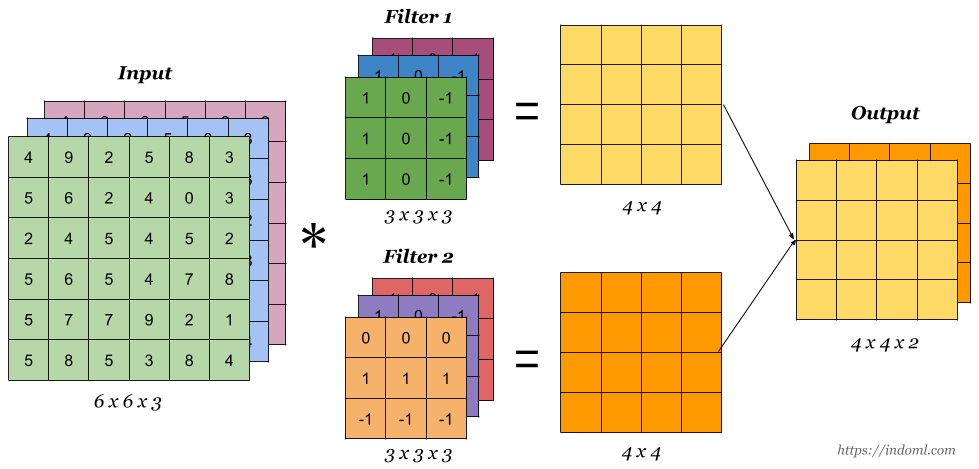
\includegraphics[width=4cm]{images/CNN_filters.png}
\caption{Trading Strategy}
\label{trading_strategy}
\end{center}
\end{figure}

One trading strategy is channels pictured in \ref{trading_strategy}

\subsection{Formula}
sdsd 
\subsubsection{subsub}
sdsd

\LaTeX{} is the program we are using right now
it is good to write 
\begin{align}
E=mc^2
\end{align}






\end{document}